\chapter{Volba a návrh periferií}

\section{LED osvětlení}

\section{Senzor teploty}

\section{Senzor výšky hladiny}

\section{Senzor pH}

\section{Ovládání 230V periferií}
%    \textit{    TODO: vybrán GPIO expandér (https://www.laskakit.cz/pcf8574-i2c-8bit-i-o-expander) a relé modul, řízeno přímo z ESP32 -- je to v jedné krabici, tak je zbytečně složité tam dávat další MCU. } 

Jak vyplývá z~požadavků zařízení a přehledu používané akvaristické techniky, pro automatizovaný provoz akvária je nutné umožnit řídící jednotce ovládat několik okruhů se síťovým napětím a spínat tak zvlášť zakoupené hotové spotřebiče pracující s~tímto napětím. Jedná se typicky o~ohřev vody, filtr, popř. některé druhy osvětlení. 

\begin{figure}[h!]
    \centering
    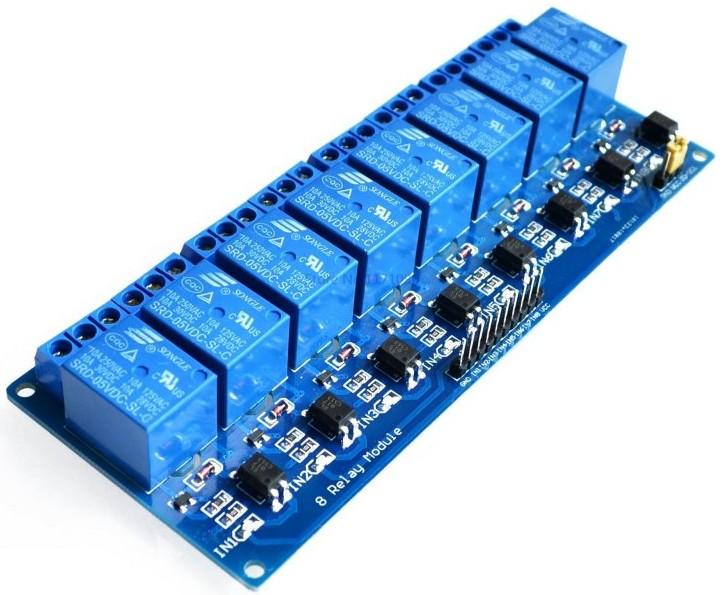
\includegraphics[width=0.6\textwidth]{obrazky/230/rele.jpg}
    \caption{Relé modul, ilustrační foto. Převzato z~\cite{eshop-laskakit-rele}.}
    \label{fig:obrazky-230-rele-jpg}
\end{figure}

\begin{figure}[h!]
    \centering
    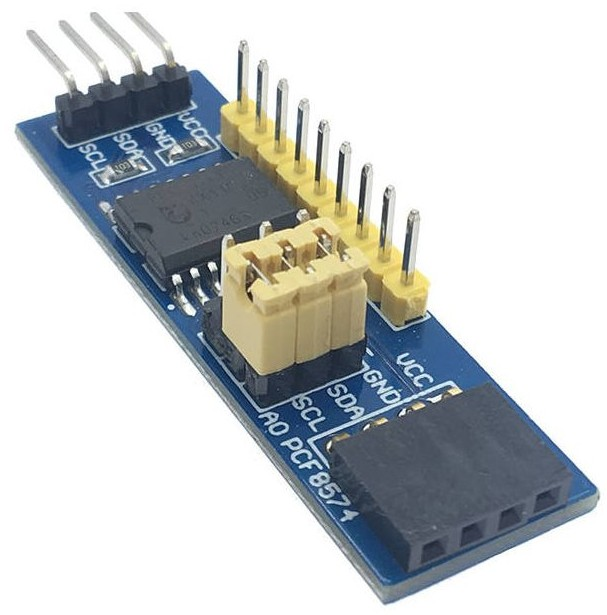
\includegraphics[width=0.4\textwidth]{obrazky/230/expander.jpg}
    \caption{Modul expandéru GPIO pinů, ilustrační foto. Převzato z~\cite{eshop-laskakit-expander}.}
    \label{fig:obrazky-230-expander-jpg}
\end{figure}

Aby uživatel mohl zařízení bezpěčně zapojit bez nutnosti odborné způsobilosti, budou se na hlavním šasi zařízení nacházet čtyři standartní zásuvky (typ E) s~jednofázovým napětím \qty{230}{V}. Fázové vodiče budou uvnitř zařízení přerušeny spínacími relé. Bude použit předpřipravený modul disponující osmi relé,kupříkladu modul na obr.~\ref{fig:obrazky-230-rele-jpg}. Zbylé čtyři relé slouží jako rezerva pro případ poškození některého z~používaných relé nebo při potřebě rozšíření o~další zásuvky. 

Z~důvodu nedostatku pinů na mikrokontroleru řídící jednotky (ESP32) bude k~relé modulu připojen ještě jeden externí modul a to expandér GPIO pinů komunikující přes sběrnici \acs{i2c}~\cite{eshop-laskakit-expander}, ilustrační foto na obr.~\ref{fig:obrazky-230-expander-jpg}. Z~pohledu mikrokontroleru tak budou všechny \qty{230}{V} zásuvky řízeny pomocí dvou datových pinů (SDA, SCL), které je navíc možné dále využít pro připojení jiných periferií jako např. OLED displaye pro zobrazení stavu zařízení. 

Možným zlepšením a rozšířením práce by bylo také zahrnutí obou zmíněných modulů přímo na DPS řídící jednotky. 


